\documentclass[11pt, onecolumn]{article}

% ─── Packages ───────────────────────────────────────────────
\usepackage[margin=1in]{geometry}
\usepackage{times}
\usepackage{amsmath, amssymb}
\usepackage{booktabs}
\usepackage{graphicx}
\usepackage[hidelinks]{hyperref}
\usepackage[numbers, sort&compress]{natbib}
\usepackage{float}
\usepackage{caption}
\usepackage{microtype}
\usepackage{xcolor}
\usepackage{array}
\usepackage{multirow}
\usepackage{setspace}
\usepackage{titlesec}
\usepackage{abstract}
\usepackage{pgf-pie}
\usepackage{tikz}

% ─── Section formatting ──────────────────────────────────────
\titleformat{\section}{\large\bfseries}{{\thesection.}}{0.5em}{}[\titlerule]
\titleformat{\subsection}{\normalsize\bfseries}{{\thesubsection}}{0.5em}{}
\titleformat{\subsubsection}{\normalsize\itshape}{{\thesubsubsection}}{0.5em}{}

% ─── Colors ──────────────────────────────────────────────────
\definecolor{stravaOrange}{HTML}{FC4C02}
\definecolor{darkgray}{HTML}{3C3C3C}

% ─── Hyperlink colors ────────────────────────────────────────
\hypersetup{
    colorlinks=true,
    linkcolor=darkgray,
    citecolor=stravaOrange,
    urlcolor=stravaOrange
}

% ─── Caption style ───────────────────────────────────────────
\captionsetup{font=small, labelfont=bf, margin=10pt}

% ─── Line spacing ────────────────────────────────────────────
\setstretch{1.05}

% ─────────────────────────────────────────────────────────────
\begin{document}

% ─── Title Block ─────────────────────────────────────────────
\begin{titlepage}
\centering
\vspace*{2cm}
{\huge\bfseries Sport Activity Classification\\[0.3cm]
Using Strava Wearable Data}\\[0.4cm]
{\large\itshape Machine Learning I --- Final White Paper}\\[0.5cm]
{\normalsize March 10, 2026}\\[2cm]
{\large
Oliver Gladfelter \\[0.3cm]
Camille Dominique Javier \\[0.3cm]
Alekhya Katreddy \\[0.3cm]
Stephanie Li \\[0.3cm]
Estella Hu \\[0.3cm]
Sola Shin \\[0.3cm]
}
\vfill
{\small Submitted in partial fulfillment of course requirements\\
Machine Learning I --- University of Chicago}
\end{titlepage}

% ─── Abstract ────────────────────────────────────────────────
\begin{abstract}
Fitness platforms like Strava require athletes to manually select their activity 
type before recording a workout --- a small but consequential friction point that 
leads to mislabeled sessions, corrupted performance statistics, and skewed 
personal records. This paper presents a supervised machine learning approach to 
automatically classifying sport activities using aggregate GPS and sensor-derived 
workout metrics, with the goal of enabling smarter, developer-friendly activity 
detection pipelines that do not depend on raw inertial sensor streams or 
proprietary hardware.

Using 397,913 real-world activities recorded by 347 athletes across 6 continents, 
we engineer 18 features from per-workout Strava data --- spanning movement 
intensity, GPS trace geometry, temporal patterns, and hemisphere-aware seasonal 
flags --- and train five classification models across the complexity spectrum: 
Logistic Regression, Decision Tree, Random Forest, Gradient Boosting, 
HistGradientBoosting, and XGBoost. The target variable consists of five grouped 
sport classes: Ride, Run, Walk, Hike, and Workout.

Our best model, a tuned XGBoost classifier, achieved a test accuracy of 91.8\% 
and a macro F1-score of 0.844 on the internal test set, generalizing to 88.9\% 
accuracy and 0.784 macro F1 on a held-out external cohort of 2,315 activities 
from a separate athlete population. SHAP-based feature importance analysis 
identified speed, movement efficiency (\texttt{moving\_time\_per}), distance, 
and GPS trace geometry (\texttt{sprawl}, \texttt{turns\_per\_mile}) as the most 
discriminating signals across activity types. The primary classification 
challenge throughout was the minority Hike class, which shares significant 
feature overlap with Walk and represents only 2.9\% of the dataset.

This work demonstrates that consumer GPS data --- without raw accelerometer 
streams or heart rate signals --- is sufficient to reliably classify the vast 
majority of sport activities. The full pipeline is reproducible and designed to 
be accessible to independent developers and sports analytics practitioners 
building on top of fitness platform APIs.
\end{abstract}

\newpage
\tableofcontents
\newpage

% ═══════════════════════════════════════════════════════════════
\section{Introduction}

\subsection{Purpose of the Study and Target Audience}

This paper presents a supervised machine learning approach to automatically 
classifying sport activities recorded on the Strava fitness platform. While the 
immediate output is a classification model, the broader purpose is to demonstrate 
that aggregate GPS and sensor-derived workout metrics are sufficient to reliably 
infer activity type --- a finding with direct implications for how fitness 
technology is designed, built, and studied. This work is directed at three 
primary audiences.

\textbf{Fitness app developers and independent software developers} are the 
primary intended audience. Developers building workout logging applications, 
training analytics tools, or third-party Strava integrations face a recurring 
challenge: users frequently mislabel their activities, either by selecting the 
wrong sport type before recording or by failing to stop a session before entering 
a vehicle. Unlike large technology companies with dedicated ML infrastructure, 
independent developers rarely have the resources to collect and label hundreds of 
thousands of activities from scratch. This study offers a reproducible, 
open-source-friendly classification pipeline --- trained on 397,913 real-world 
workouts --- that developers can build on directly. The feature engineering 
methodology, particularly the GPS trace geometry features (\texttt{turns\_per\_mile}, 
\texttt{wobble}, \texttt{sprawl}), is designed to be implementable using data 
already available through the Strava API and equivalent fitness platforms.

\textbf{Data scientists and machine learning practitioners} working in sports 
analytics, athlete performance modeling, or the broader quantified-self space 
represent a second key audience. Most published Human Activity Recognition (HAR) 
research relies on raw inertial sensor streams from controlled laboratory 
settings \citep{attal2015}. This study contributes an alternative perspective: 
demonstrating that per-workout aggregate features, derived entirely from 
consumer GPS devices in real-world conditions, are sufficient to achieve 91.8\% 
accuracy and 0.844 macro F1 across five activity classes at scale. The SHAP-based 
interpretability framework and external validation methodology are designed to be 
reproducible and adaptable to similar classification problems in sports and 
activity recognition research.

\textbf{Athletes and quantified-self enthusiasts} form the downstream 
beneficiary group --- the end users who stand to gain most from tools built on 
this research. Competitive athletes who rely on Strava for performance tracking 
are directly affected when a mislabeled workout corrupts their pace history, 
training load metrics, or personal records. Casual users who simply want an 
accurate record of their activity are similarly impacted. While this paper is 
technical in nature, the problem it addresses is immediately familiar to anyone 
who has accidentally started a cycling session on a running profile, or forgotten 
to stop their watch before driving home. The practical applications of this 
work --- automatic activity correction, anomaly flagging, and smarter defaults 
in recording interfaces --- are ultimately in service of this audience.

\subsection{What is Strava?}

Strava is a social fitness platform and activity tracker with over 120 million registered users worldwide. Athletes use Strava to record, share, and analyze their workouts across a wide range of sport types, including running, cycling, hiking, walking, and gym-based activities. Each workout is logged with GPS trace data, movement metrics (distance, speed, elevation), and temporal metadata (date, time). Strava's open API makes it a valuable source of large-scale, real-world fitness data, and its community-driven design means the dataset captures genuine behavioral diversity across athlete types, geographic regions, and device ecosystems.

\subsection{Scope and Limitations}

This study is scoped to five grouped sport classes---\textbf{Ride, Run, Walk, Hike, and Workout}---derived from Strava's native taxonomy of approximately 50 sport types. Several limitations apply: first, the dataset consists of \textbf{per-workout aggregate metrics} rather than raw inertial sensor streams (accelerometer, gyroscope), which are more commonly used in academic Human Activity Recognition (HAR) research. This constrains the granularity of movement signals available to the model. Second, the study relies on user-provided activity labels as ground truth, which introduces label noise since users can occasionally mislabel their own workouts. Third, class imbalance---Hike represents only 2.9\% of the dataset---persistently limits classification performance for that class across all models evaluated. Finally, the dataset is sourced from a self-selected population of Strava users, which may not be representative of the global athletic population.

% ═══════════════════════════════════════════════════════════════
\section{Literature Review}

Human Activity Recognition (HAR) has been an active research domain for over two decades, driven initially by healthcare applications such as fall detection and rehabilitation monitoring, and more recently by the commercialization of consumer wearables. The core challenge in HAR is to map sensor or GPS data onto discrete activity categories using statistical or machine learning models.

Traditional machine learning approaches dominated early HAR research. Methods such as Support Vector Machines (SVM), k-Nearest Neighbors (k-NN), and Hidden Markov Models were applied to hand-crafted features extracted from accelerometer and gyroscope signals. These approaches required significant domain expertise in feature engineering but produced interpretable, computationally lightweight models well-suited for deployment on low-power devices.

A systematic review covering HAR literature from 2021 to 2024 \citep{islam2025} found that the field has shifted substantially toward deep learning, with Convolutional Neural Networks (CNN), Long Short-Term Memory (LSTM) networks, and Transformer architectures now representing the state of the art for raw sensor stream classification. However, the same review noted that \textbf{ensemble tree-based methods remain competitive on tabular, aggregate-level feature sets}---precisely the data format used in this study.

\citet{yuan2024} demonstrated in \textit{npj Digital Medicine} that self-supervised learning on 700,000 person-days of UK Biobank accelerometer data could produce generalizable HAR models with macro F1 improvements of up to 130\% over supervised baselines on external datasets. While their approach leveraged raw inertial signals at a scale far exceeding this study, their findings highlight the importance of dataset diversity and generalization testing---motivating our own external validation step.

The Sussex-Huawei Locomotion and Transportation Mode Recognition (SHL) Challenge \citep{wang2023shl} specifically targets GPS and motion sensor data for classifying locomotion and transportation modes---the closest academic analog to our problem. Top-performing SHL submissions consistently used gradient boosted tree ensembles combined with GPS-derived spatial features, supporting our feature engineering choices around route geometry (turns per mile, wobble, sprawl).

For the modeling framework, XGBoost \citep{chen2016xgboost} has become the dominant algorithm for supervised classification on structured tabular data since its introduction. It employs second-order gradient optimization, built-in L1/L2 regularization, and histogram-based split finding, making it substantially faster than standard gradient boosting while achieving comparable or superior accuracy.

A closely related prior study---a Strava-based fitness analysis project \citep{mocchicone2020}---applied Logistic Regression and SVM to activity data from two athletes. While methodologically similar in spirit, that work's small sample size (528 records) limits its generalizability. Our study extends this line of work to nearly 400,000 activities across 347 athletes, introducing richer GPS-derived features, ensemble boosting models, SHAP-based interpretability, and external validation.

% ═══════════════════════════════════════════════════════════════
\section{Data and Features}

\subsection{Data Overview}

The dataset consists of 398,442 Strava activities recorded by 347 unique athletes. Each row represents one complete workout session. After removing 529 anomalous activities (0.13\% of the dataset), 397,913 clean observations were retained for modeling. Athletes contributed an average of approximately 1,148 activities each, though individual counts varied substantially.

The geographic distribution spans 6 continents, with approximately 80\% of activities originating from the Northern Hemisphere and 20\% from the Southern Hemisphere. Device diversity is broad: Garmin devices account for the largest share, followed by Apple Watch, the Strava mobile app, COROS, Zwift, Suunto, and Wahoo, among others. This heterogeneity across athletes, geographies, and devices reduces the risk that the model learns device-specific or region-specific artifacts.

\begin{figure}[H]
    \centering
    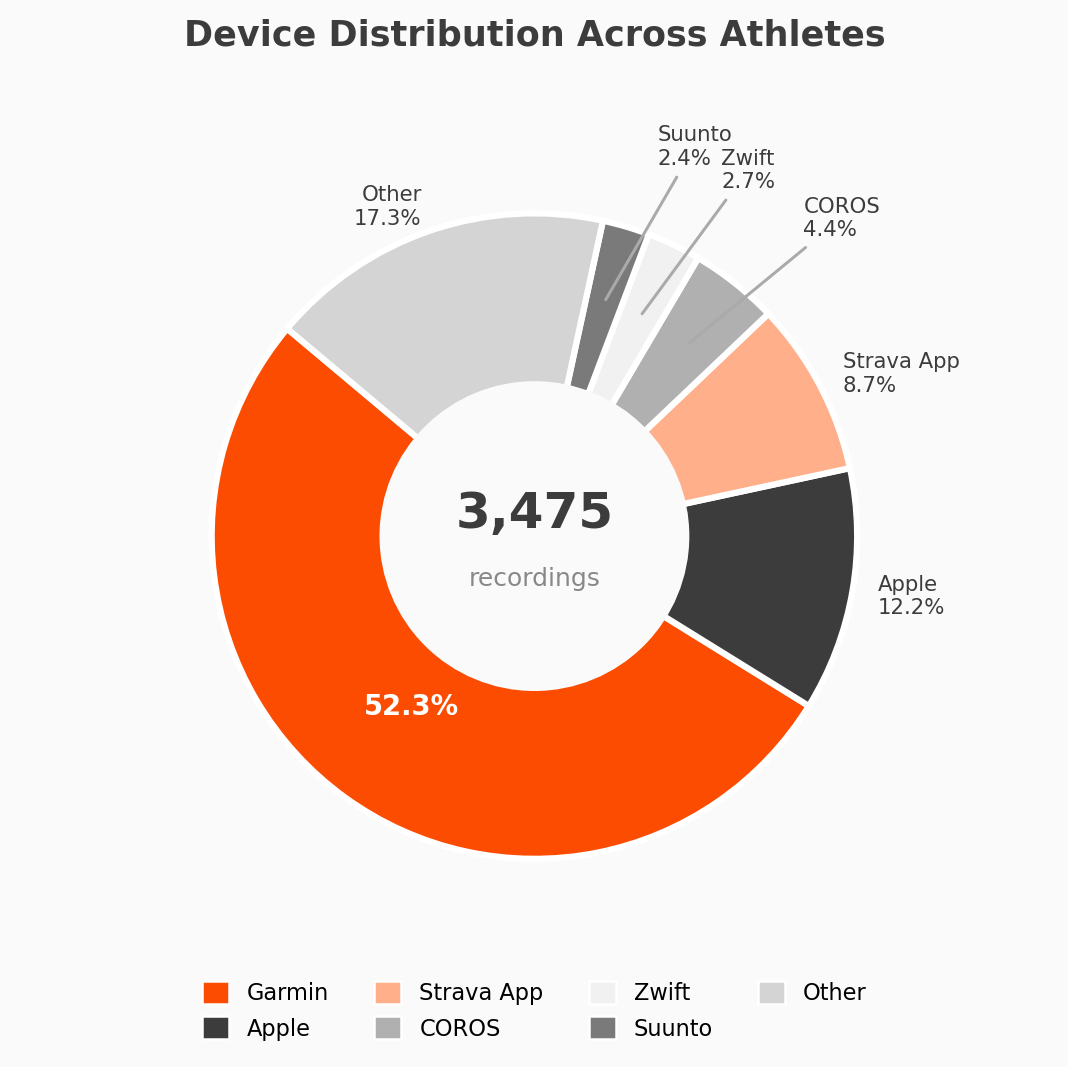
\includegraphics[width=0.8\textwidth]{device_distribution_chart}
    \caption{Device distribution across 347 athletes. ``Other'' includes Wahoo, Polar, Nike,
Samsung, and 18 additional platforms each representing less than 2\% of recordings.}
    \label{fig:Device Distribution by Brand}
\end{figure}

\textbf{Target variable:} The raw Strava data contains approximately 50 unique sport types. These were grouped into five categories: \textbf{Ride} (42\%), \textbf{Run} (37\%), \textbf{Workout} (9\%), \textbf{Walk} (9\%), and \textbf{Hike} (3\%). Table~\ref{tab:classes} summarizes the class distribution.

\begin{table}[H]
\centering
\caption{Target class distribution and distinguishing characteristics.}
\label{tab:classes}
\begin{tabular}{llp{7cm}}
\toprule
\textbf{Class} & \textbf{\% of Dataset} & \textbf{Key Characteristics} \\
\midrule
Ride    & 42\% & High speed, long distance, low turns/mile, high sprawl \\
Run     & 37\% & Moderate speed and distance, high \texttt{moving\_time\_per} \\
Workout &  9\% & Near-zero elevation, often no GPS, indoor setting \\
Walk    &  9\% & Low speed, high turns/mile, shorter distance \\
Hike    &  3\% & High elevation gain, low speed, low \texttt{moving\_time\_per} \\
\bottomrule
\end{tabular}
\end{table}

\subsection{Missing Data and Anomaly Handling}

Two features were dropped due to high missingness: \texttt{suffer\_score} (82\% missing, subscriber-only) and \texttt{device\_name} (84\% missing). Four GPS-derived features---\texttt{num\_turns}, \texttt{turns\_per\_mile}, \texttt{wobble}, and \texttt{sprawl}---were missing for 14\% of activities, structurally indicating GPS-free workouts. These were zero-filled and a binary indicator \texttt{has\_gps} was added.

Anomaly detection combined DBSCAN (on a 25,000-activity sample) with a rule-based speed threshold of 32 mph---the approximate legal e-bike maximum. Activities exceeding this threshold were flagged and removed (529 total, $<$0.13\%).

\begin{figure}[H]
    \centering
    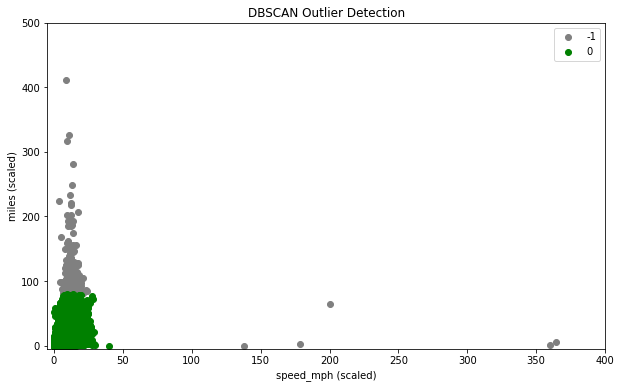
\includegraphics[width=0.7\textwidth]{dbscan_output}
    \caption{DBSCAN on about 6\% of the entire dataset to determine speed thresholds and boundaries.}
    \label{fig:DBSCAN Outlier Detection on a Sample Set}
\end{figure}

\subsection{Feature Engineering}

The final model feature set consists of 18 variables across four conceptual categories.

\subsubsection{Core Movement Metrics}

\begin{itemize}
    \item \texttt{speed\_mph}: average speed computed as miles divided by elapsed time in 
    hours. Speed above 32 mph was used as the anomaly detection threshold.
    
    \item \texttt{miles}: total distance in miles, consolidated from redundant 
    \texttt{distance} and \texttt{kilometers} columns.
    
    \item \texttt{moving\_time}: total seconds of active movement, excluding pauses 
    such as rest stops or traffic lights.
    
    \item \texttt{elapsed\_time}: total session duration in seconds, including all pauses.
    
    \item \texttt{moving\_time\_per}: ratio of \texttt{moving\_time} to 
    \texttt{elapsed\_time}. Captures how continuously the athlete moved --- hikers 
    show lower values due to rest breaks, while runners show the highest.
    
    \item \texttt{feet\_per\_mile}: elevation gain normalized by distance. A key 
    discriminator between Hike (high) and Workout (near-zero).
\end{itemize}

\subsubsection{GPS Trace Geometry}

\begin{itemize}
    \item \texttt{has\_gps}: binary flag indicating GPS availability. Zero-fills were 
    applied to all GPS-derived features for non-GPS activities (e.g.\ indoor workouts, 
    treadmill runs).
    
    \item \texttt{num\_turns}: total number of directional changes along the GPS trace.
    
    \item \texttt{turns\_per\_mile}: turns normalized by distance. Rides have few turns 
    per mile due to long straight roads; Walks have many due to short neighborhood loops.
    
    \item \texttt{wobble}: tortuosity of the GPS trace --- measures how curved versus 
    straight the recorded path was.
    
    \item \texttt{sprawl}: diagonal of the bounding box around the GPS trace, serving 
    as a proxy for how geographically spread-out the activity was.
\end{itemize}

\subsubsection{Temporal Features}

\begin{itemize}
    \item \texttt{hour}: start hour of the workout (0--23).
    
    \item \texttt{month}: calendar month of the workout.
    
    \item \texttt{dayofweek}: day of the week (0 = Monday, 6 = Sunday).
    
    \item \texttt{is\_weekend}: binary flag for Saturday and Sunday. Hikers skew 
    heavily toward weekend activity.
    
    \item \texttt{is\_winter} / \texttt{is\_summer}: hemisphere-aware seasonal flags 
    constructed from \texttt{month} and \texttt{is\_northern\_hemisphere}, ensuring 
    seasons are not inverted for Southern Hemisphere athletes.
\end{itemize}

\subsubsection{Categorical Feature}

\begin{itemize}
    \item \texttt{day\_part}: time-of-day binned into four categories --- morning, 
    afternoon, evening, and night. One-hot encoded in the preprocessing pipeline. 
    Hikers are almost exclusively morning athletes; night activity is rare across 
    all outdoor classes.
\end{itemize}

\subsection{Exploratory Data Analysis}

Kruskal-Wallis tests and Dunn post-hoc comparisons were run on all continuous features; chi-squared tests were applied to binary and categorical features. Key findings:

\begin{itemize}
    \item \textbf{\texttt{speed\_mph}} is the strongest single discriminator. Ride is statistically distinct from all classes ($p \approx 0$). Hike and Walk overlap significantly.
    \item \textbf{\texttt{feet\_per\_mile}} sharply separates Hike (high elevation) from Workout (near-zero). Less useful for Ride, Run, Walk.
    \item \textbf{\texttt{moving\_time\_per}} confirms that hikers take more breaks. Hike shows the lowest distribution; Runs show the highest.
    \item \textbf{\texttt{turns\_per\_mile}} and \textbf{\texttt{wobble}} are highly correlated. Rides have far fewer turns per mile than Walks.
    \item \textbf{\texttt{is\_weekend}} distinguishes Hike clearly from all other classes.
    \item \textbf{Critical finding:} Hike vs.\ Walk is the most persistent source of misclassification. Elevation gain and \texttt{is\_weekend} are the primary discriminating signals but insufficient alone for high Hike recall.
\end{itemize}

% ═══════════════════════════════════════════════════════════════
\section{Methodology}

\subsection{Data Preparation and Train/Test Split}

Data was collected from Strava's public API and split 80/20 into training (318,330 activities) and test (79,583 activities) sets using stratified sampling to preserve class proportions. A separate external validation set of 2,315 activities from a distinct athlete cohort was held out entirely and used only for out-of-sample generalization testing. 

\subsection{Preprocessing Pipeline}

All models were implemented within a \texttt{scikit-learn} \texttt{Pipeline} to prevent data leakage. A \texttt{ColumnTransformer} applied one-hot encoding (\texttt{drop='first'}) to \texttt{day\_part} and passthrough for all numeric features. \texttt{StandardScaler} was applied downstream for Logistic Regression only; tree-based models received no scaling as decision tree splits are invariant to feature magnitude.

\subsection{Models}

\subsubsection{Logistic Regression}
Implemented as the linear baseline with \texttt{max\_iter=1000} to ensure convergence. This model serves as a reference for how much non-linear modeling adds relative to a simple interpretable model. 

\subsubsection{Decision Tree}
A single decision tree serving as a non-linear but non-ensemble baseline. This model was tuned via \texttt{GridSearchCV} over a  \texttt{max\_depth} $\in \{10, 20, \text{None}\}$, \texttt{min\_samples\_split} $\in \{2, 10\}$, and split criterion (Gini vs. Entropy)  using 3-fold cross-validation optimizing macro F1 score.

\subsubsection{Random Forest}
A bagging ensemble of 200 trees, addressing the variance instability of the prior single decision tree. \texttt{GridSearchCV} optimized \texttt{max\_depth}, \texttt{max\_features} (sqrt vs log2), and \texttt{n\_estimators}.

\subsubsection{Gradient Boosting}
A sequential boosting ensemble, serving as the baseline boosting model. This model utilizes \texttt{RandomizedSearchCV} over 25 configurations searched \texttt{n\_estimators} $\in [100, 500]$, \texttt{learning\_rate} $\in \{0.03, 0.05, 0.1\}$, \texttt{max\_depth} $\in \{2, 3, 4\}$, and \texttt{subsample} $\in \{0.6, 0.8, 1.0\}$, with the subsample parameter enabling stochastic gradient boosting to reduce overfitting.

\subsubsection{HistGradientBoosting}
Scikit-learn's histogram-based boosting variant with early stopping enabled, chosen for its reliability for large datasets and histogram binning capabilities for continuous variables to reduce split-finding complexity. In this model we use \texttt{RandomizedSearchCV} over 20 configurations covered \texttt{learning\_rate}, \texttt{max\_depth}, \texttt{max\_leaf\_nodes}, \texttt{min\_samples\_leaf}, and L2 regularization.

\subsubsection{XGBoost}
Extreme Gradient Boosting (XGBoost) was the primary candidate model, given its established dominance for structured tabular classification tasks. This model is configured with \texttt{objective='multi:softprob'}, \texttt{tree\_method='hist'}, and \texttt{eval\_metric='mlogloss'}. \texttt{RandomizedSearchCV} over 20 configurations with 3-fold \texttt{StratifiedKFold} optimized macro F1. The best configuration was:

\begin{table}[H]
\centering
\footnotesize
\caption{Tuned XGBoost hyperparameter configuration.}
\label{tab:xgb_params}
\begin{tabular}{llp{8cm}}
\toprule
\textbf{Parameter} & \textbf{Value} & \textbf{Rationale} \\
\midrule
\texttt{n\_estimators}      & 800   & Large ensemble captures complex decision boundaries \\
\texttt{max\_depth}         & 8     & Deep trees model non-linear feature interactions \\
\texttt{learning\_rate}     & 0.1   & Moderate shrinkage balances speed and generalization \\
\texttt{subsample}          & 0.6   & Stochastic sampling reduces overfitting to dominant classes \\
\texttt{colsample\_bytree}  & 1.0   & All features considered at each tree split \\
\texttt{min\_child\_weight} & 1     & Minimal leaf constraint allows fine-grained splits \\
\texttt{reg\_lambda}        & 0.5   & L2 regularization penalizes large leaf weights \\
\texttt{objective}          & \texttt{multi:softprob} & Probabilistic multi-class output \\
\texttt{tree\_method}       & \texttt{hist}           & Histogram-based split finding for large datasets \\
\texttt{eval\_metric}       & \texttt{mlogloss}       & Multinomial log-loss for multi-class evaluation \\
\bottomrule
\end{tabular}
\end{table}

\subsection{Evaluation Metrics}

Given class imbalance (Hike at 2.9\%), accuracy alone is insufficient. All models were evaluated on:
\begin{itemize}
    \item \textbf{Test Accuracy}: proportion of correctly classified activities.
    \item \textbf{Macro F1-score}: unweighted mean of per-class F1 scores. Primary comparison metric.
    \item \textbf{Per-class precision, recall, F1}: from full classification reports.
    \item \textbf{Confusion matrix}: to analyze misclassification patterns.
\end{itemize}

% ═══════════════════════════════════════════════════════════════
\section{Results}

\subsection{Model Performance Comparison}

Table~\ref{tab:model_comparison} summarizes performance across all models on the internal test set.

\begin{table}[H]
\centering
\caption{Internal test set performance comparison.}
\label{tab:model_comparison}
\begin{tabular}{lcccp{5cm}}
\toprule
\textbf{Model} & \textbf{Accuracy} & \textbf{Macro F1} & \textbf{Hike F1} & \textbf{Notes} \\
\midrule
Logistic Regression      & 0.845 & 0.720 & 0.42 & Linear baseline \\
Decision Tree            & 0.883 & 0.797 & 0.51 & High variance \\
Random Forest            & 0.911 & 0.836 & 0.58 & Best non-boosting model \\
Gradient Boosting        & 0.906 & 0.828 & 0.62 & Strong on dominant classes \\
HistGradientBoosting     & 0.910 & 0.832 & 0.61 & Efficient; comparable to GBM \\
\textbf{XGBoost (Tuned)} & \textbf{0.918} & \textbf{0.844} & \textbf{0.63} & Best overall \\
\bottomrule
\end{tabular}
\end{table}

XGBoost achieved the highest performance on every metric. The macro F1 gap between Logistic Regression (0.720) and XGBoost (0.844) demonstrates the substantial non-linear structure in the data that linear models cannot capture. Hike F1 improved progressively with model complexity, peaking at 0.63.

\subsection{External Validation}

The tuned XGBoost model was applied to a held-out external dataset of 2,315 activities from a separate cohort. Table~\ref{tab:external} reports the comparison.

\begin{table}[H]
\centering
\caption{XGBoost internal test vs.\ external validation performance.}
\label{tab:external}
\begin{tabular}{lccc}
\toprule
\textbf{Dataset} & \textbf{Accuracy} & \textbf{Macro F1} & \textbf{Hike F1} \\
\midrule
Internal Test Set    & 0.9179 & 0.8441 & 0.63 \\
External Validation  & 0.8886 & 0.7844 & 0.38 \\
\bottomrule
\end{tabular}
\end{table}

Generalization was strong for high-support classes: Ride (F1: 0.92), Run (F1: 0.92), Walk (F1: 0.84), and Workout (F1: 0.86) remained consistent with internal benchmarks. The Hike class showed the most pronounced degradation (F1: 0.38 vs.\ 0.63 internally), driven by extremely low external support ($n=49$) and persistent feature overlap with Walk.

\subsection{Error Analysis}

The top misclassification pairs in external evaluation are:

\begin{itemize}
    \item \textbf{Ride $\rightarrow$ Run} (45 instances): overlapping speed/distance at moderate cycling intensities.
    \item \textbf{Workout $\rightarrow$ Run} (30 instances): heterogeneous workouts with running-like kinematics.
    \item \textbf{Hike $\rightarrow$ Walk} (28 instances): structural ambiguity between low-intensity outdoor activities.
    \item \textbf{Walk $\rightarrow$ Run} (26 instances): edge cases at the pace boundary.
    \item \textbf{Walk $\rightarrow$ Hike} (22 instances): hilly walk routes resembling hikes by elevation profile.
\end{itemize}

\subsection{Feature Importance via SHAP}

SHAP (SHapley Additive exPlanations) values were computed on a stratified sample of 500 test observations using \texttt{PermutationExplainer}. Global feature importance was derived as:

\begin{equation}
\bar{\phi}_j = \frac{1}{NK} \sum_{i=1}^{N} \sum_{k=1}^{K} |\phi_{ijk}|
\label{eq:shap}
\end{equation}

where $i$ indexes samples, $j$ features, and $k$ classes. \texttt{speed\_mph} ranked first by a substantial margin under both SHAP and XGBoost gain importance, followed by \texttt{moving\_time\_per}, \texttt{miles}, \texttt{sprawl}, and \texttt{feet\_per\_mile}.

Notable divergences between SHAP and gain importance were observed for binary features. \texttt{has\_gps} ranked 4th by gain but 14th by mean absolute SHAP---consistent with the known tendency of gain to inflate the apparent importance of binary features with skewed distributions. SHAP provides a more representative measure by averaging contributions across all observations.

\begin{figure}[H]
    \centering
    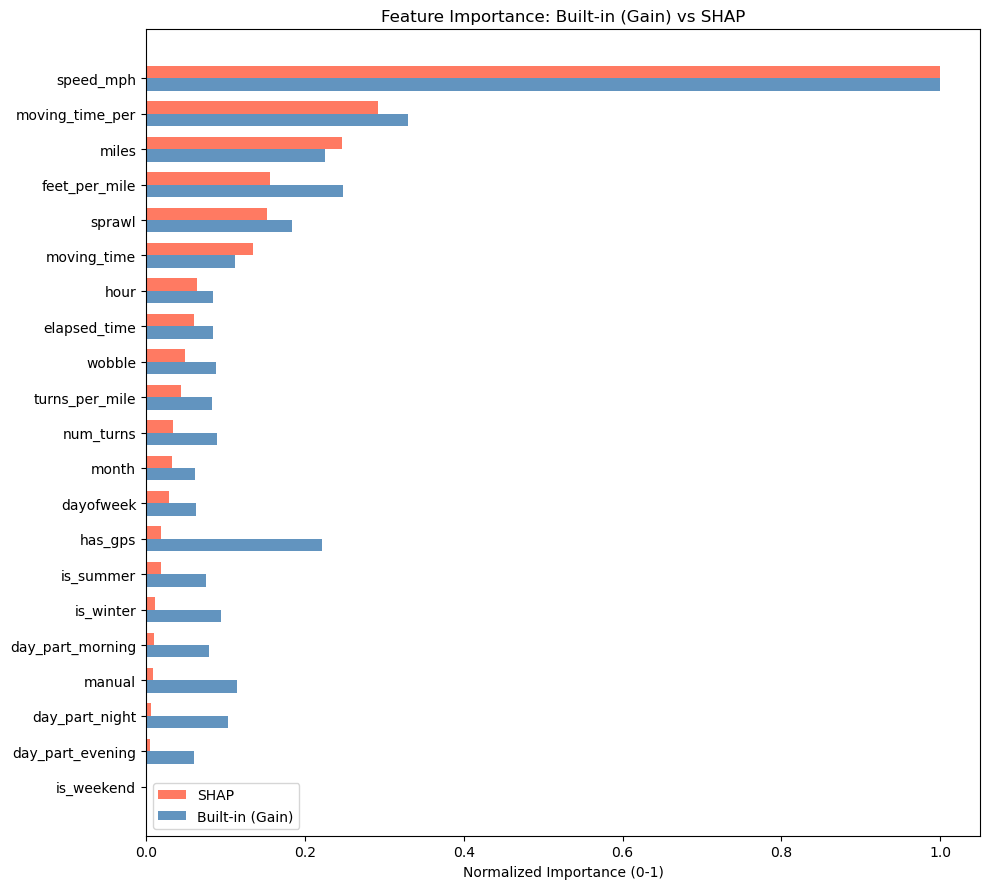
\includegraphics[width=0.9\textwidth]{shap.png}
    \caption{Feature Importance Comparison using SHAP and Gain}
    \label{fig:SHAP Analysis}
\end{figure}

% ═══════════════════════════════════════════════════════════════
\section{Conclusions and Future Work}

\subsection{Summary of Findings}

This study demonstrated that aggregate workout metrics from consumer GPS devices are sufficient to reliably classify five sport activity types. The tuned XGBoost classifier achieved 91.8\% accuracy and 0.844 macro F1 on the internal test set, generalizing to 88.9\% accuracy and 0.784 macro F1 on an external cohort. Speed, movement efficiency, distance, and GPS trace geometry emerged as the most discriminating features. The Hike class remained persistently difficult due to feature overlap with Walk, low sample prevalence, and activity heterogeneity.

\subsection{Future Extensions}

\begin{itemize}
    \item \textbf{Hike/Walk disambiguation}: targeted features such as elevation gain rate, route linearity index, and maximum sustained gradient could resolve the most persistent confusion pair.
    \item \textbf{Class rebalancing}: SMOTE or class-weighted training to improve minority class recall.
    \item \textbf{Raw GPS trace modeling}: sequence-based models (LSTM, CNN) on decoded polylines could capture route shape information lost in aggregation.
    \item \textbf{Athlete persona clustering}: unsupervised segmentation of athletes into behavioral personas (competitive runner, casual cyclist, weekend hiker) using aggregate workout history.
    \item \textbf{E-bike detection}: a binary classifier targeting the Ride vs.\ E-Bike boundary using speed-elevation profile signatures.
    \item \textbf{Real-time inference}: a streaming version classifying activity type from a rolling window of GPS data during the workout, enabling on-device auto-correction.
\end{itemize}

% ═══════════════════════════════════════════════════════════════
\section*{Author Contributions or Acknowledgements}
The authors used Claude (Anthropic, 2025) and Gemini (Google DeepMind, 2025) to assist with code development and manuscript drafting. All outputs were reviewed and edited by the authors.

\bibliographystyle{apalike}
\nocite{*}
\bibliography{references}

\end{document}